\documentclass[bachelor,german]{hgbthesis}
% Zul�ssige Class Options: 
%   Typ der Arbeit: diplom, master (default), bachelor, praktikum 
%   Hauptsprache: german (default), english
%%------------------------------------------------------------

\graphicspath{{images/}}    % wo liegen die Bilder?
\AddBibFile{literatur.bib}  % Angabe der BibTeX-Datei

%%%----------------------------------------------------------
\begin{document}
%%%----------------------------------------------------------

% Eintr�ge f�r ALLE Arbeiten: --------------------------------
\title{Erkennung, Verfolgung und Klassifizierung von Schiffen
und Booten auf der Spree anhand des Videostreams einer IP-Kamera}
\author{Marcel Schwittlick}
\studiengang{Angewandte Informatik}
\studienort{HTW Berlin}
\abgabedatum{2013}{02}{05}	% {YYYY}{MM}{DD}

%% f�r Bachelorarbeit und Praktikumsbericht entsprechende Eintr�ge erg�nzen:

%%% zus�tzlich f�r eine Bachelorarbeit: ---------------------
\nummer{s0529494}   % XX...X = Stud-ID, z.B. 0310238045-A  
                        % (A = 1. Bachelorarbeit)
\semester{Wintersemester 2013 / 2014} 
\gegenstand{Bachelor Thesis} 
\betreuer{Prof. Dr. Frank ~Bauern�ppel, Prof. Dr. Albrecht Fortenbacher} % oder \betreuerin{..}

\strictlicense  % erzeugt restriktive Lizenzformel

%%%----------------------------------------------------------
\frontmatter
\maketitle
\tableofcontents
%%%----------------------------------------------------------

\chapter{Vorwort} 	% engl. Preface



Dies ist \textbf{Version \hgbthesisDate} der \latex-Dokumentenvorlage f�r 
verschiedene Abschlussarbeiten an der FH Hagenberg, die mittlerweile auch 
an anderen Hochschulen im In- und Ausland gerne verwendet wird.

Das Dokument entstand urspr�nglich auf Anfragen von Studierenden,
nachdem im Studienjahr 2000/01 erstmals ein offizieller
\latex-Grundkurs im Studiengang Medientechnik und -design an der
FH Hagenberg angeboten wurde. Eigentlich war die Idee, die bereits
bestehende \emph{Word}-Vorlage f�r Diplomarbeiten "`einfach"' in
\latex\ zu �bersetzen und dazu eventuell einige spezielle
Erg�nzungen einzubauen. Das erwies sich rasch als wenig
zielf�hrend, da \latex, \va was den Umgang mit Literatur und
Graphiken anbelangt, doch eine wesentlich andere Arbeitsweise
verlangt. Das Ergebnis ist -- von Grund auf neu geschrieben und
wesentlich umfangreicher als das vorherige Dokument --
letztendlich eine Anleitung f�r das Schreiben mit \latex, erg�nzt
mit einigen speziellen (mittlerweile entfernten) Hinweisen f�r \emph{Word}-Benutzer.
Technische Details zur aktuellen Version finden sich in Anhang \ref{ch:TechnischeInfos}.

W�hrend dieses Dokument anfangs ausschlie�lich f�r die Erstellung
von Diplomarbeiten gedacht war, sind nunmehr auch  
\emph{Masterarbeiten}, \emph{Bachelor\-arbeiten} und \emph{Praktikumsberichte} 
abgedeckt, wobei die Unterschiede bewusst gering gehalten wurden.

Bei der Zusammenstellung dieser Vorlage wurde versucht, mit der
Basisfunktionalit�t von \latex das Auslangen zu finden und -- soweit m�glich --
auf zus�tzliche Pakete zu verzichten. Das ist nur zum Teil gelungen;
tat\-s�ch\-lich ist eine Reihe von erg�nzenden "`Paketen"' notwendig, wobei jedoch
nur auf g�ngige Erweiterungen zur�ckgegriffen wurde.
Selbstverst�ndlich gibt es dar�ber hinaus eine Vielzahl weiterer Pakete,
die f�r weitere Verbesserungen und Finessen n�tzlich sein k�nnen. Damit kann
sich aber jeder selbst besch�ftigen, sobald das notwendige Selbstvertrauen und
gen�gend Zeit zum Experimentieren vorhanden sind.
Eine Vielzahl von Details und Tricks sind zwar in diesem Dokument nicht explizit
angef�hrt, k�nnen aber im zugeh�rigen Quelltext jederzeit ausgeforscht
werden.

Zahlreiche KollegInnen haben durch sorgf�ltiges Korrekturlesen und
konstruktive Verbesserungsvorschl�ge wertvolle Unterst�tzung
geliefert. Speziell bedanken m�chte ich mich bei Heinz Dobler f�r
die konsequente Verbesserung meines "`Computer Slangs"', bei
Elisabeth Mitterbauer f�r das bew�hrte orthographische Auge und
bei Wolfgang Hochleitner f�r die Tests unter Mac~OS.

Die Verwendung dieser Vorlage ist jedermann freigestellt und an
keinerlei Erw�hnung gebunden. Allerdings -- wer sie als Grundlage
seiner eigenen Arbeit verwenden m�chte, sollte nicht einfach
("`ung'schaut"') darauf los werken, sondern zumindest die
wichtigsten Teile des Dokuments \emph{lesen} und nach M�glichkeit
auch beherzigen. Die Erfahrung zeigt, dass dies die Qualit�t der
Ergebnisse deutlich zu steigern vermag.


Der Quelltext zu diesem Dokument sowie das zugeh�rige
\latex-Paket sind in der jeweils aktuellen Version online
verf�gbar unter
%
\begin{quote}
\url{www.fh-hagenberg.at/staff/burger/diplomarbeit/}
%\href{www.fh-hagenberg.at/staff/burger/diplomarbeit/}{www.fh-hagenberg.at/staff/burger/diplomarbeit/}
\end{quote}
%
oder auch unter
%
\begin{quote}
\url{http://elearning.fh-hagenberg.at/} \newline
im Kurs "`Anleitung/Vorlage f�r Master-/Bachelor-/Diplomarbeiten"'.
%\url{http://theses.fh-hagenberg.at}
\end{quote}
%
Trotz gro�er M�he enth�lt dieses Dokument zweifellos Fehler und Unzul�nglichkeiten
-- Kommentare, Verbesserungsvorschl�ge und passende Erg�nzungen
sind daher stets willkommen, am einfachsten per E-Mail direkt an mich:
\begin{center}%
\begin{tabular}{l}
\nolinkurl{wilhelm.burger@fh-hagenberg.at} \\
Dr.\ Wilhelm Burger \\
FH Hagenberg -- Digitale Medien\\
Austria
\end{tabular}
\end{center}

\noindent
�brigens, hier im Vorwort (das bei Diplomarbeiten �blich, bei Bachelorarbeiten 
aber entbehrlich ist) kann man kurz auf die Entstehung  des Dokuments eingehen.
Hier ist auch der Platz f�r allf�llige Danksagungen (\zB an den Betreuer, 
den Begutachter, die Familie, den Hund, ...), Widmungen und philosophische 
Anmerkungen. Das sollte man allerdings auch nicht �bertreiben und sich auf 
einen Umfang von maximal zwei Seiten beschr�nken.




		% ggfs. weglassen
\chapter{Kurzfassung}
Diese Bachelorarbeit besch�ftigt sich mit der Aufgabenstellung anhand eines Bildsequenz Objekte zu erkennen und zu verfolgen. Diese Bildsequenz soll anhand einer IP-Kamera aufgezeichnet werden, damit sie �ber das Internet von jedem Ort der Welt ausgewertet werden kann.
Bei den Objekten, die zu erkennen und verfolgen sind handelt es sich um Schiffe und Boote auf einem Fluss. 

Zus�tzlich soll untersucht werden, ob und wenn ja, inwiefern die erkannten Objekte klassifiziert werden k�nnen, um gegebenenfalls Muster im Schiffsverkehr erkennen zu k�nnen. M�gliche Anhaltspunkte f�r Klassifikatoren k�nnen Eigenschaften der Schiffe, wie Typ, Gr��e, und Geschwindigkeit sein.

Der praktische Teil dieser Arbeit soll aus einem Prototypen bestehen, welche den gefunden L�sungsansatz demonstriert. Dieser Prototyp soll aus einer Hardware- und einer Softwarekomponente bestehen.

Die Erkennung, Verfolgung und Klassifizierung soll mittels bekannter und bereits implementierter Computer Vision Algorithmen geschehen und es soll untersucht werden, inwiefern das System m�glichst robust gegen�ber Wettereinfl�ssen erstellt werden kann. Es soll ein theoretischer Ansatz zur Klassifikation der Schiffe entwickelt werden, welche nicht teil der praktischen Arbeit sein soll.
\chapter{Abstract}
The main goal of the Bachelor thesis is to detect and track ships and boats on a live video stream. Further it is to research by which properties the boats can be classified, in order to 
create some sort of patterns and statistics about the traffic on the river. 
The hardware of the system needs to be developed, in order to create a weatherproff installation of the camera. The prototype is supposed to be portable to any other part of the river, whereas the system needs to be adjustablable to other environments, like different lighting, weather and viewpoint situations. 
The detection and recognition of the boats is going to be implemented using known and common computer vision algorithms and is supposed to be resistent to different weather infliences. For classifying the boats, methods of machine learning are supposed to be researched and compared to other approaches.

%%%----------------------------------------------------------
\mainmatter         % Hauptteil (ab hier arab. Seitenzahlen)
%%%----------------------------------------------------------

\chapter{Einleitung}
In den folgenden Kapiteln wird beschrieben, wiö das Problem dieser Bachelor Arbeit angegangen wurde.

\begin{enumerate}
\item \textbf{Einführung }: Was ist die Problem- oder Aufgabenstellung und warum sollte man sich dafür interessieren?
\item \textbf{Analyse / Präzisierung des Themas}:Zunächst wird die Aufgabe näher analysiert. Hier beschreibt man den aktuellen Stand der Technik oder Wissenschaft ("`State-Of-The-Art"'), zeigt bestehende
							Defizite oder offene Fragen auf und entwickelt daraus die Sto\ss{}richtung der eigenen Arbeit.
\item \textbf{Definition}:Daraus ergibt sich eine Definition des Problemes und der naechsten Handlungsschritte.
\item \textbf{Grundlagen}:Dann werden die Grundlagen der Definierten Ziele beschrieben.
\item \textbf{Entwurf / Eigener Ansatz}:Anschliessend wird ein Entwurf des zu entwickelnden Systemes dargelegt.
\item \textbf{Implementierung / Prototyp}:Woraus eine tatsaechliche Implementierung resuliert.
\item \textbf{Test}:Welche getestet werden muss.
\item \textbf{Fazit / Zusammenfassung}:Und durch ein Fazit abgerundet wird.
\end{enumerate}

\section{Motivation}
Für die Entwicklung solche eines Systemes gibts es für den Autor dieser Arbeit diverse Motivationen. Das wichtigste Motiv ist es dem Autor eine Möglichkeit zu geben sich umfangreich und selbstständig mit dem Thema der Computer Vision zu beschäftigen. Die Thematik Informationen über Objekte und deren Zusammenhang anhand von Bildern und Bildersequenzen zu gelangen faszinierte den Autor bereits seit einiger Zeit. Weiterhin hatte der Autor noch nie die Gelegenheit sich mit der Thematik des Maschinellen Lernens auseinanderzusetzen, wo diese Arbeit das Potenzial bietet gro\ss{}en gebrauch davon zu machen.
Im Zusammenhang damit steht, dass der Autor von den Neuigkeiten und Nachrichten bezüglich der \"Uberwachungssysteme im In- und Ausland verwirrt ist und mit eigenen Fähigkeiten herausfinden möchte, inwiefern diese \"Uberwachungssysteme tatsächlich funktionieren und wozu sie in der Lage sind. In den Nachrichten wurde in den letzten Jahren verhäuft über Städte(London) und Situationen(Terroranschlag Boston) berichtet. Dazu möchte der Autor herausfinden, wozu solche Systeme technisch in der Lage sind, und was für einen potenziellen Gewinn an Sicherheit sie versprechen können.

\"Uber diese persönliche Motivation hinaus bietet die Entwicklung eines solchen Systemes gro\ss{}en \"Okonomischen Wert, da dadurch Statistiken und Informationen über den Schiffsverkehr an unterschiedlichen Stellen des gleichen Flusses verglichen werden können, um daraus Schlüsse über ??? zu ziehen.

\section{Relevanz}
\section{Aufbau der Arbeit}
\chapter{Anforderungsanalyse}
In der Bachelorarbeit soll es darum gehen Schiffe bzw. Boote anhand eines Live-Videostreames zu erkennen und zu tracken. Zus�tzlich soll untersucht werden, inwiefern die Schiffe nach bestimmten
Kriterien klassifiziert werden k�nnen, um gegebenenfalls Muster im Flussverkehr erkennen zu
k�nnen. M�gliche Klassifikatoren k�nnen der Schifftyp, die Gr��e des Schiffes und die
Geschwindigkeit des Schiffes sein. Dadurch k�nnen detaillierte Statistiken �ber einen bestimmten
Flussabschnitt erstellt werden, welche gegebenenfalls mit Statistiken anderer Flussabschnitte
verglichen werden k�nnen. 
Deswegen soll die Hardwarekomponente des Systemes portabel und
resistent gegen�ber Wettereinfl�ssen sein. Die Entwicklung der Hardware Komponente soll
ebenfalls Teil der Arbeit sein und aus einer IP-Kamera inklusive Wetterresistenter Halterung
bestehen. Es soll ein funktionierender Prototyp erarbeitet werden, der mit wenigen Schritten an
einen anderen Ort umgezogen werden kann. Dies erfordert h�chstwarscheinlich eine Art
Kalibrierung des Systemes auf die ver�nderten Umgebungsfaktoren, wie Blickwinkel und
Lichtverh�ltnisse des neuen Ortes, welche elementarer Teil des Systemes sein soll.
Die Erkennung, Verfolgung und Klassifizierung soll mittels bekannter und bereits implementierter
Computer Vision Algorithmen geschehen und m�glichst robust gegen�ber eventuellen
Wettereinfl�ssen sein. Zur Klassifizierung der Schiffe soll die Methode des Maschinellen Lernens in
Betracht gezogen werden, allerdings mit anderen Ans�tzen zur Klassifizierung verglichen werden.
Es soll eine Software entwickelt werden, welche es erm�glicht Schiffe anhand von digitalem Videosignal zu erkennen, zu verfolgen und zu klassifizieren. Dieses Problem ist ein Klassisches Problem der Computer Vision und mit den n�tigen Methoden und Mitteln umzusetzen. Allerdings soll die Software weiterhin f�r die M�glichkeit die Kamera an verschieden Orte zu stellen gestaltet werden. Durch die unterschiedlichen Positionen der Kamera muss die Software variablen gebaut sein, sodass man das System an die ge�nderten Umst�nde anpassen kann. Weiterhin muss bedacht werden, dass das Software system zu jeder Zeit w�hrend des Tages funktionieren soll und muss sich deswegen an �ndernde Wetterumst�nde anpassen k�nnen, oder so robust gebaut sein, dass sie zu jeder Jahreszeit funktioniert.

\section{Anwendungsgebiet}
Die Arbeit besch�ftigt sich mit der Thematik anhand von Bildern und Bildsequenzen ( Videos ) aussagekr�ftige Informationen zu erhalten. Ein Bild repr�sentiert im Computer speicher ist nichts weiter, als eine
Matrix mit bestimmter H�he und Breite, welche multipliziert die Pixelanzahl des Bildes angeben. An jeder Position dieser Matrix sind die Farbwerte zu dem entsprechendem Pixel gespeichert. Durch die Betrachtung dieser Pixelmatrix kann unser menschliches Gehirn ohne weiteres dem Bild Informationen �ber dessen Inhalt entnehmen, folglich das Bild zu interpretieren. Die Interpretation eines Bildes ist ein komplexes Konstrukt und ist durch unsere Erfahrung als Mensch m�glich. Mehr zu diesem Thema in einem abgesonderten Block.
Ein Computer hat allerdings kein komplexes Gehirn und sieht ein Bild, was f�r einen Menschen z.B. gro�en emotionalen Wert haben kann schlichtweg als einen zweidimensionalen Array, welcher konkrete farbwerte enth�lt.
Anhand dieser repr�sentation des Bildes kann allerdings der Computer instruiert werden bestimmte Muster zu erkennen, oder bestimmte Operationen auf das Bild anzuwenden, wodurch letztendlich dem Bild Informationen 
entnommen werden kann. Diese Verarbeitung wird maschinelles Sehen oder Bildverstehen engl. Computer Vision genannt und besch�ftigt sich damit computergest�tzt Bilder auf eine menschliche Art und Weise zu interpretieren. Das Thema maschinelles Sehen wird im Abschnitt Maschinelles Sehen n�her beschrieben.

\section{Umsetzung}
\section{Anforderungen an den Prototypen}
Der Prototyp soll in der Lage sein unter m�glichst allen Wetterumst�nden Schiffe anhand des Videostreames der IP-Kamera zu erkennen. Dies soll nur tags�ber passieren.
Dieser Prototyp soll an unterschiedlichen Orten eingesetzt werden k�nnen, gegebenenfalls soll die Kamera an einen anderen Flussabschnitt bewegt werden k�nnen und die Software soll an die dort gegebenen lokalen Umst�nde anpassbar sein. Diese Anpassung soll anhand einer Grafischen Benutzeroberfl�che geschehen.
\subsection{Hardware}
Die Hardwarekomponente des Prototypen soll aus einer Kamera bestehen, die entweder Videosinal �ber das Netzwerk / Internet an den verarbeitenden Rechner inkl. Software sendet, oder direkt an einem Computer angeschlossen sein, welcher die Verarbeitung dann direkt vor Ort vornimmt. Allerdings ergibt sich dadurch das Problem, dass ein Computer am FLuss stehen mnuss, was nicht immer m�glich ist, da eine Stromzufuhr nicht immer gegeben sein kann. ( Wie soll denn �berhaupt eine Kamera dort funktionieren? Eventuell eine Kamera per Batterie laufen lassen mit Mobilem Hotspot?!! ) 

\subsubsection{Kamera}
An die Kamera, die die Aufgabe hat den Flussausschnitt zu filmen werden nur wenige Anforderungen gestellt. Sie soll ausschlie�lich die F�higkeit haben ihren Videostream �ber das Internet erreichbar zu machen. Die Qualit�t des Videostreames ist ein Kriterium, das ausser Acht gelassen werden soll.
Als Kamera wurde die AXIS M1031-M gew�hlt, da sie schlichtweg gegeben war und den Anforderungen entspricht. Sie bietet ihren Stream in diversen Formaten ( h.264, Motion JPEG, MPEG-4 ) an und war bereits eingerichtet.
Ausserdem hat diese Kamera den Vorteil einer einfachen Installation, einer 640x480 Pixel Aufl�sung mit einer Bildrate von 30FPS.

\begin{figure}
\centering
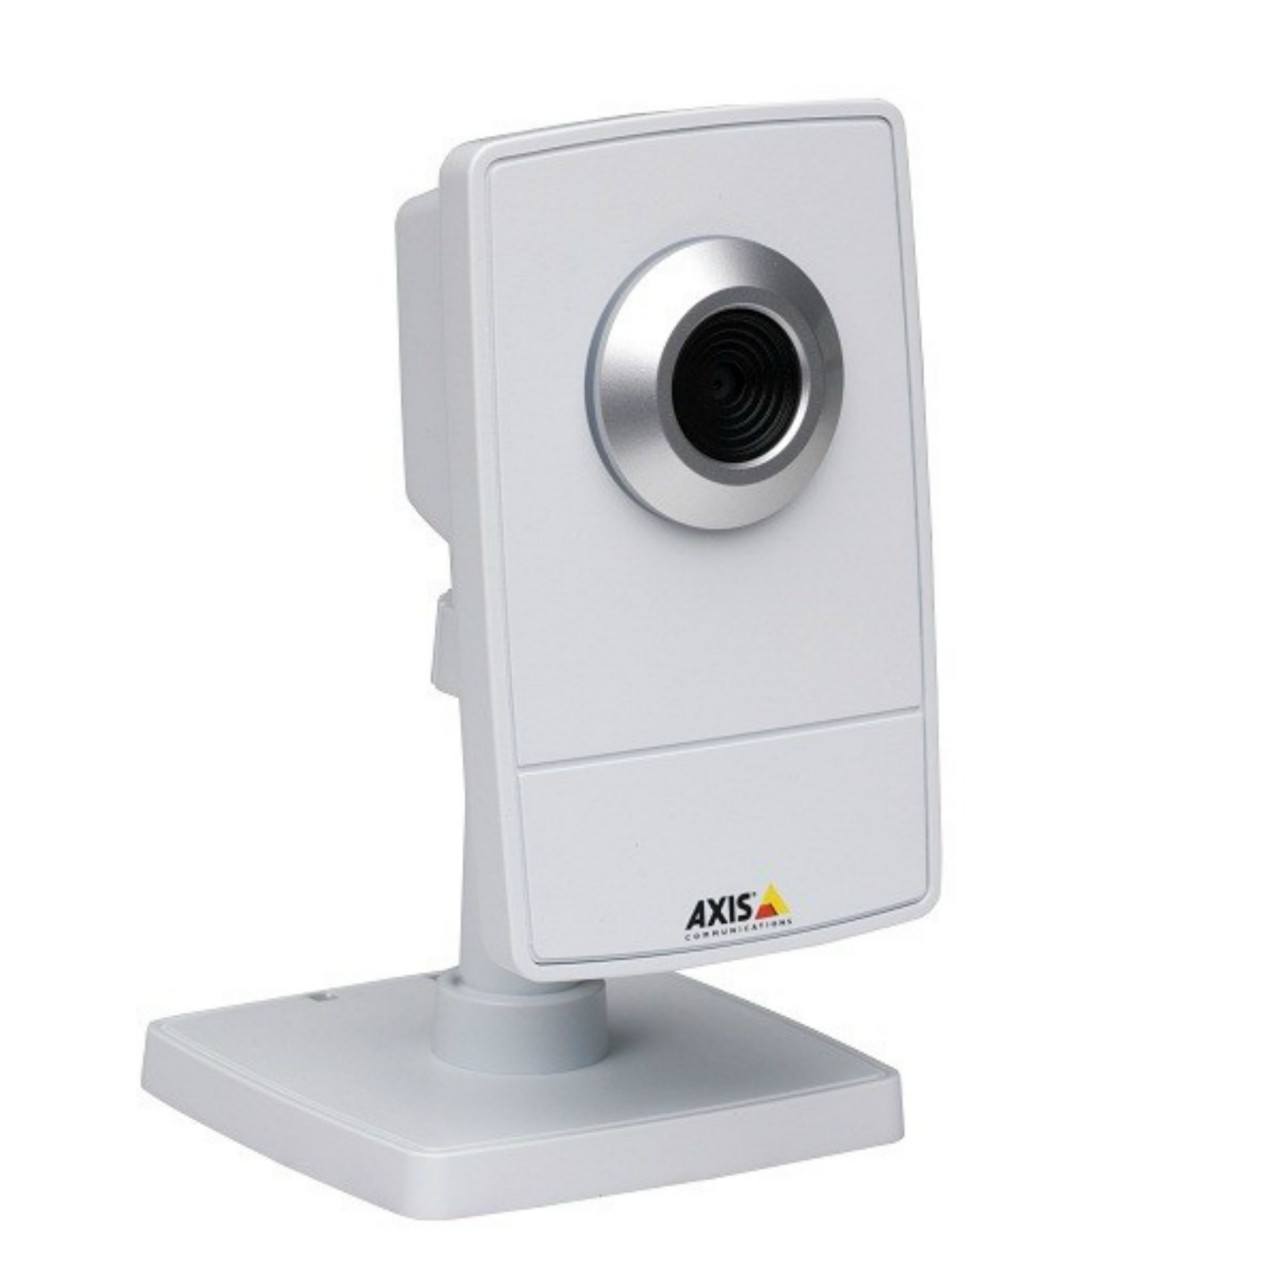
\includegraphics[width=.95\textwidth]{axis_camera} %{CS0031}
\caption[AXIS M1031-M]{AXIS M1031-M\footnotemark}
\label{fig:AXIS M1031-M}
\end{figure}
\subsubsection{Halterung}
\subsubsection{Benutzte Hardware}
\subsection{Software}
\footnotetext{\url{http://www.networkcamerastore.com/axis-m1031-w-0300-004-wireless-network-camera}}
Die Softwarekomponente des Systemes soll inder Lage sein aus einer erh�hren Position am Flussrand Schiffe zu erkennen, zu verfolgen und gegebenenfalls klassifizieren und sonstige Informationen �ber das Schiff, wie z.B. Geschwindigkeit, L�nge aufzuzeichnen. Die Position aus der die Kamera auf den Fluss 'sieht' soll variabel sein und die Sofware soll an diese ver�nderbaren Umst�nde angepasst werden k�nnen. Diese Anpassung soll anhand einer grafischen Benutzeroberfl�che geschehen k�nnen.
\subsubsection{Benutzeroberfl�che}
Die grafische Benutzeroberfl�che soll es dem Benutzer erm�glichen die Algorithmen, die zur Erkennung und Verfolgung der Schiffe bnuetzt werden fein zu parametrisieren. Dazu sollen alle entscheidenden Parameter der Algorithmen aoffen gelegt werden und durch Standard Oberfk�chen-Elemente ver�nderbar sein.
\subsubsection{Performance}
Da die Verarbeitung des Videostreames in Echtzeit geschehen soll die Software alle m�glichen Parallelisierungsmethoden benutzen, die sich anbieten. 
\section{Abgrenzungskriterien}
In diesem Abschnitt wird erl�utert von welchen Anforderungen sich der Prototyp klar abgrenzt. Dar�ber sollte ich mir mal gedanken machen-
\section{Methodik}
In den folgenden Unterabschnitten wird tiefer auf die Umsetzung des Prototypen und dieser Dokumentation eingegangen. Es werden Hilfsmittel, die das Projektmanagement und die Programmierung unterst�tzen gegeneinander abgewogen und untersucht.
\subsection{Projektmanagement}
Um ein professionelles und strukturiertes Projektmanagement zu gew�hrleisten muss ich f�r eine Unterst�tzung entschieden werden. G�ngige M�glichkeiten bieten Projektmanagement-Systeme wie trac und Redmine.
\begin{figure}
\centering
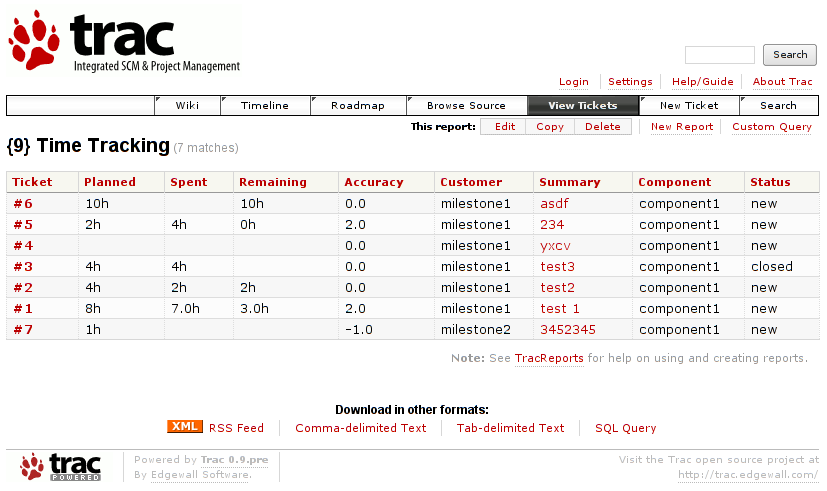
\includegraphics[width=.95\textwidth]{trac-timetracking-report} %{CS0031}
\caption[trac Projektmanagement]{trac Projektmanagement\footnotemark}
\label{fig:trac Projektmanagement}
\end{figure}
\subsection{Programmiermethodik}
\footnotetext{\url{http://trac.edgewall.org/wiki/TimeTracking}}
Bei diesem Projekt kann kein nicht-iteratives Vorgehensmodell, wie das Wasserfallmodell benutzt werden, da sich die tats�chlichen Anforderungen an die Software erst w�hrend der Implementierungsphase herausstellen. Man kann bei solch einem Projekt vorab schlichtweg nicht sagen, welche Bildverarbeitungsmethoden genau angewandt werden sollen, da nach der Implementierung zun�chst eine fundierte Untersuchung der Ergebnisse geschehen muss, um zu entscheiden, welche Folgeverarbeitungen darauf aufbauen k�nnen. Es gibt diverse Ans�tze, die das Problem dieser Arbeit l�sen, welche jedoch nicht vor tats�chlicher Implementierung festgehalten werden k�nnen.
Daher wurde sich entschieden eine agile Vorgehensweise zu w�hlen, um genau diese Art des Projektes zu addressieren. Dadurch kann sich unmittelbar an Erkenntnisse der Implementierung angepasst werden.
\subsubsection{Agile Programmierung}
\subsubsection{Extreme Programming}

\chapter{Zukunftsaussichten}
F�r die Zukunft k�nnte ein System entwickelt werden, welches Schiffe sogar ausgesprochen schnell auf kosteng�nstiger Hardware erkannt werden k�nnte. Dieser Ansatzt spaltet das gesammte System in zwei Teile. Diese beiden Teile sind jeweils voneinander abgekoppelte Applikationen, wobei die erstApplikation im gro�en und ganzen der in dieser AStbeit beschriebenen gleicht. Der entscheidende Unterschied jodoch liegt darin, dass diese Sofware nicht unmittelbar daf�r benutzt wird, Schiffe zu erkennen und zu tracken, sondern lediglich daf�r benutzt wird einen Machine-Learning Algorithmus wie z.B. den Haar-Classifier zu trainieren. Dadurch kann die Software nach kurzer vorangegangener Parameterkalibierung eigenst�ndig Bilder von Schiffen erkennen und speichern, welche darauf zum Training des Haar-Klassifiers benutzt werden.
Der zweite Teil des Systemes w�re ein Computer mit Raspberry-Pi-�hnlicher Architektur und Leistung, welcher daf�r zust�ndig ist das digitale Videosignal ausschliesslich anhand eines Haar-Klassifiers zu analysieren, was selbst auf der heutzuztage billigsten Hardware in Echtzeit m�glich ist. (30euro RaspPi)


\end{document}